\section{5. Cálculos y resultados}
\subsection{5.1. Uso de unidades}
\begin{itemize}
  \item Unidad de la regla usada ( $\ell$ ): 1 cm
  \item Unidad de la balanza digital (m) : 1 g
  \item Unidad del pie de rey (p) : 1 mm
\end{itemize}

\subsection{5.2. Uso de cifras significativas}
\begin{itemize}
  \item Se utilizan solo hasta dos cifras decimales por cada medición realizada(En sus respectivas unidades).
  \item Se utilizan hasta 4 cifras significativas en el cálculo de áreas, esfuerzos y módulos elásticos.
\end{itemize}

\subsection{5.3. Cálculo de errores}
\begin{itemize}
  \item Error de la regla : $\Delta \ell=0,5 \mathrm{~cm}$
  \item Error de la balanza digital : $\Delta m=0,1 g$
  \item Error del pie de rey : $\Delta p=0,03 m m$
\end{itemize}

\subsection{5.4. Resultados obtenidos y comparación con otros conocidos}
\subsection{5.4.1. Tablas, gráficos y comparación con otros resultados conocidos}

\begin{table}[H]
\centering
\begin{tabular}{|c|c|c|c|c|c|c|c|c|}
\hline
   & Masa(Kg) &  Peso & Longitud & $\Delta l$ & $\epsilon$ & Area $S_o (m^2)$  & Area $S (m^2)$ & $\sigma$ \\ \hline 
  1 & 0.4958 &  & 0.216 & 0.274 &  &  &  &    \\ \hline 
  2 & 0.7502 &  & 0.216 & 0.321 &  &  &  &    \\ \hline
  3 & 1.004 &  & 0.216 & 0.370 &  &  &  &    \\ \hline 
  4 & 1.2576 &  & 0.216 & 0.416 &  &  &  &    \\ \hline 
  5 & 1.459 &  & 0.216 & 0.454 &  &  &  &    \\ \hline
  5 & 1.459 &  & 0.454 & 0.454 &  &  &  &    \\ \hline 
  4 & 1.2576 &  & 0.454 & 0.417 &  &  &  &    \\ \hline 
  3 & 1.004 &  & 0.454 & 0.370 &  &  &  &    \\ \hline 
  2 & 0.7502 &  & 0.454 & 0.321 &  &  &  &    \\ \hline 
  1 & 0.4958 &  & 0.454 & 0.274 &  &  &  &    \\ \hline
\end{tabular}
\caption{Datos de masa, peso, longitudes, áreas y presiones con diámetros correspondientes}
\label{tab:datos}
\end{table}

\begin{center}
\begin{tabular}{|l|l|l|l|l|}
\hline
 & \multicolumn{2}{|r|}{Masas ( $\Delta m=0,1 \mathrm{~g}$ )} & Longitudes $(\Delta x=0,5 \mathrm{~mm})$ & Diámetro ( $\Delta D=0,03 \mathrm{~mm})$ \\
\hline
$\mathrm{N}^{\circ}$ & Nominal & $\operatorname{Real}(\mathrm{g})$ & $\mathrm{L}\left(10^{-3} \mathrm{~m}\right)$ & $\mathrm{D}\left(10^{-3} \mathrm{~m}\right)$ \\
\hline
1 & 500 & 501.0 & 227 & 13.74 \\
\hline
2 & 750 & 755.7 & 275 & 12.67 \\
\hline
3 & 1000 & 1004.6 & 317 & 11.65 \\
\hline
4 & 1250 & 1259.3 & 362 & 10.83 \\
\hline
5 & 1500 & 1505.6 & 404 & 10.51 \\
\hline
6 & 1750 & 1760.3 & 447 & 10.19 \\
\hline
\end{tabular}
\end{center}

Cuadro 1: Tabla de datos para el resorte\\
Donde $D_{0}=14 \mathrm{~mm}, m_{\text {resorte }}=59,7 \mathrm{~g}, L_{0}=191 \mathrm{~mm}$.

\begin{center}
\begin{tabular}{|l|l|l|l|l|l|}
\hline
$\mathrm{N}^{\circ}$ & Peso(N) & $\mathrm{S}\left(10^{-6} m^{2}\right)$ & $\Delta \mathrm{L}\left(10^{-3} \mathrm{~m}\right)$ & $\sigma(\mathrm{Pa})$ & $\varepsilon$ \\
\hline
1 & 4.915 & 148,273 & 36 & 33146.936 & 0.188 \\
\hline
2 & 7.413 & 126.079 & 84 & 58799.728 & 0.440 \\
\hline
3 & 9.855 & 106.596 & 126 & 92452.881 & 0.660 \\
\hline
4 & 12.354 & 92.118 & 171 & 134106.990 & 0.895 \\
\hline
5 & 14.770 & 86.755 & 213 & 170248.502 & 1.115 \\
\hline
6 & 17.269 & 81.553 & 256 & 211747.088 & 1.340 \\
\hline
\end{tabular}
\end{center}

Cuadro 2: Valores procesados de la tabla 1

\begin{center}
\begin{tabular}{|l|l|l|l|l|l|}
\hline
 & \multicolumn{2}{|r|}{Masas ( $\Delta m=0,1 \mathrm{~g}$ )} & Longitudes $(\Delta x=0,5 \mathrm{~mm})$ & \multicolumn{2}{|c|}{Dimensiones ( $\Delta a=0,03 \mathrm{~mm}$ )} \\
\hline
$\mathrm{N}^{\circ}$ & Nominal & $\operatorname{Real}(g)$ & $\mathrm{L}\left(10^{-3} m\right)$ & $\mathrm{a}\left(10^{-3} \mathrm{~m}\right)$ & $\mathrm{b}\left(10^{-3} \mathrm{~m}\right)$ \\
\hline
1 & 500 & 501.0 & 318 & 14.60 & 5.50 \\
\hline
2 & 750 & 755.7 & 334 & 14.48 & 5.44 \\
\hline
3 & 1000 & 1004.6 & 346 & 14.42 & 5.40 \\
\hline
4 & 1250 & 1259.3 & 376 & 14.32 & 5.20 \\
\hline
5 & 1500 & 1505.6 & 398 & 14.22 & 5.18 \\
\hline
6 & 1750 & 1760.3 & 426 & 14.06 & 5.04 \\
\hline
\end{tabular}
\end{center}

Cuadro 3: Datos para liga (carga)

\begin{center}
\begin{tabular}{|l|l|l|l|l|l|}
\hline
 & \multicolumn{2}{|r|}{Masas ( $\Delta m=0,1 g$ )} & Longitudes $(\Delta x=0,5 \mathrm{~mm})$ & \multicolumn{2}{|c|}{Dimensiones ( $\Delta a=0,03 \mathrm{~mm}$ )} \\
\hline
$\mathrm{N}^{\circ}$ & Nominal & $\operatorname{Real}(g)$ & $\mathrm{L}\left(10^{-3} m\right)$ & $\mathrm{a}\left(10^{-3} \mathrm{~m}\right)$ & $\mathrm{b}\left(10^{-3} \mathrm{~m}\right)$ \\
\hline
5 & 1500 & 1505.6 & 418 & 14.12 & 5.14 \\
\hline
4 & 1250 & 1259.3 & 391 & 14.40 & 5.20 \\
\hline
3 & 1000 & 1004.6 & 362 & 14.68 & 5.30 \\
\hline
2 & 750 & 755.7 & 343 & 14.72 & 5.36 \\
\hline
1 & 500 & 501.0 & 332 & 15.06 & 5.40 \\
\hline
\end{tabular}
\end{center}

Cuadro 4: Datos para liga (descarga)\\
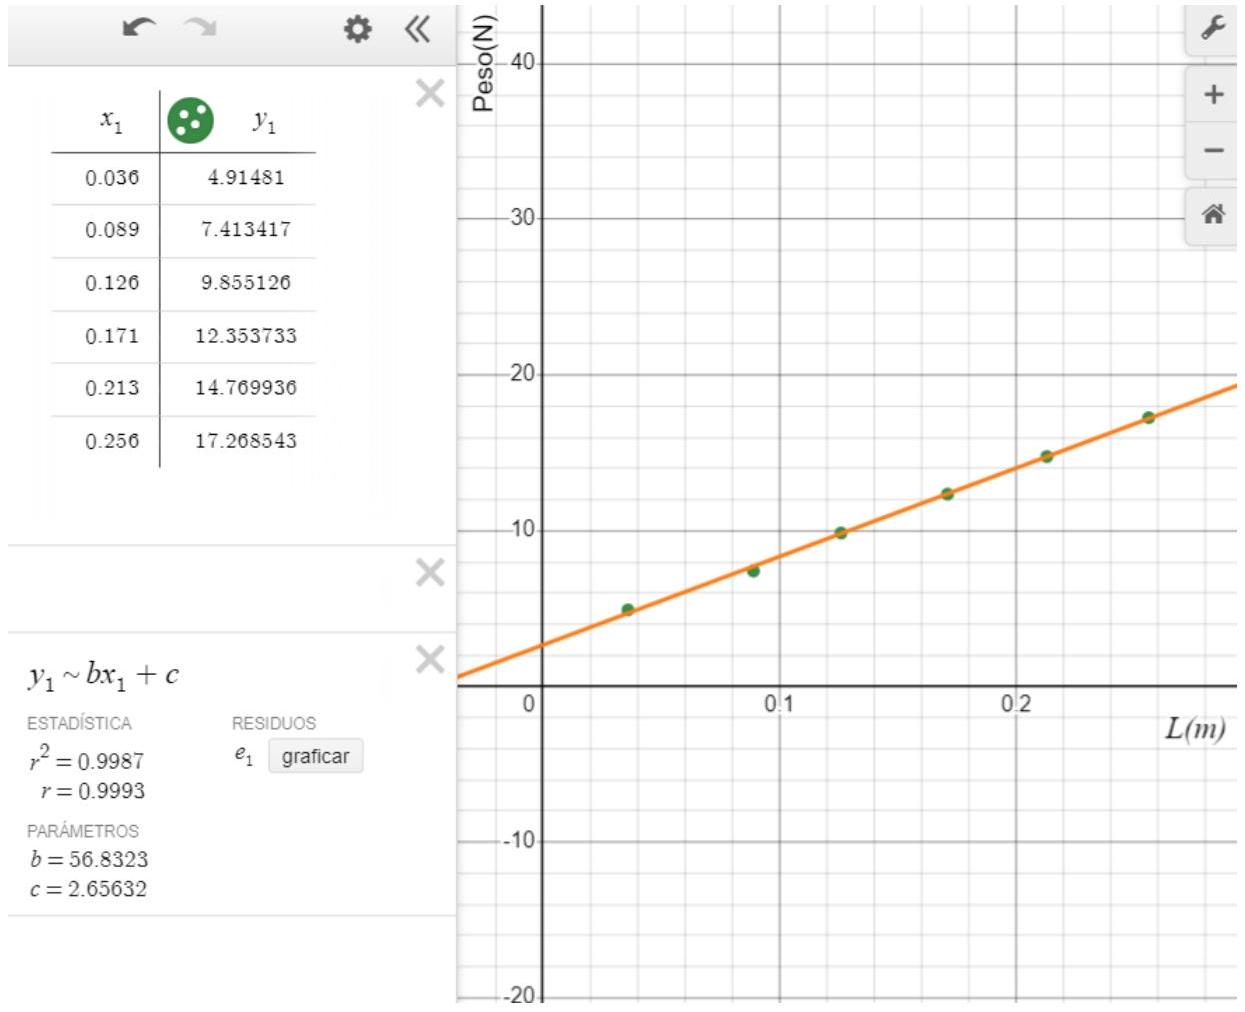
\includegraphics[max width=\textwidth, center]{2025_04_28_5f0b00b867417d4cd835g-3}

Figura 8: Gráfico F vs $\ell$

Tenemos para las tablas anteriores, que $a_{0}=15,58 \mathrm{~mm}, b_{0}=5,92 \mathrm{~mm}, m_{\text {liga }}=39,1 \mathrm{~g}$ y $L_{0}=29,6 \mathrm{~cm}$.\\
De la gráfica presente en la figura 8 , tenemos:

\begin{itemize}
  \item Se cumple la ley de Hooke(hay relación de proporcionalidad entre $F$ y $\Delta \ell$ )
  \item La constante de elasticidad viene dada por b, por lo que $k=56,8323 \frac{N}{m} \approx 56,832 \frac{N}{m}$.
  \item Se observa una precisión de 0.9987.\\
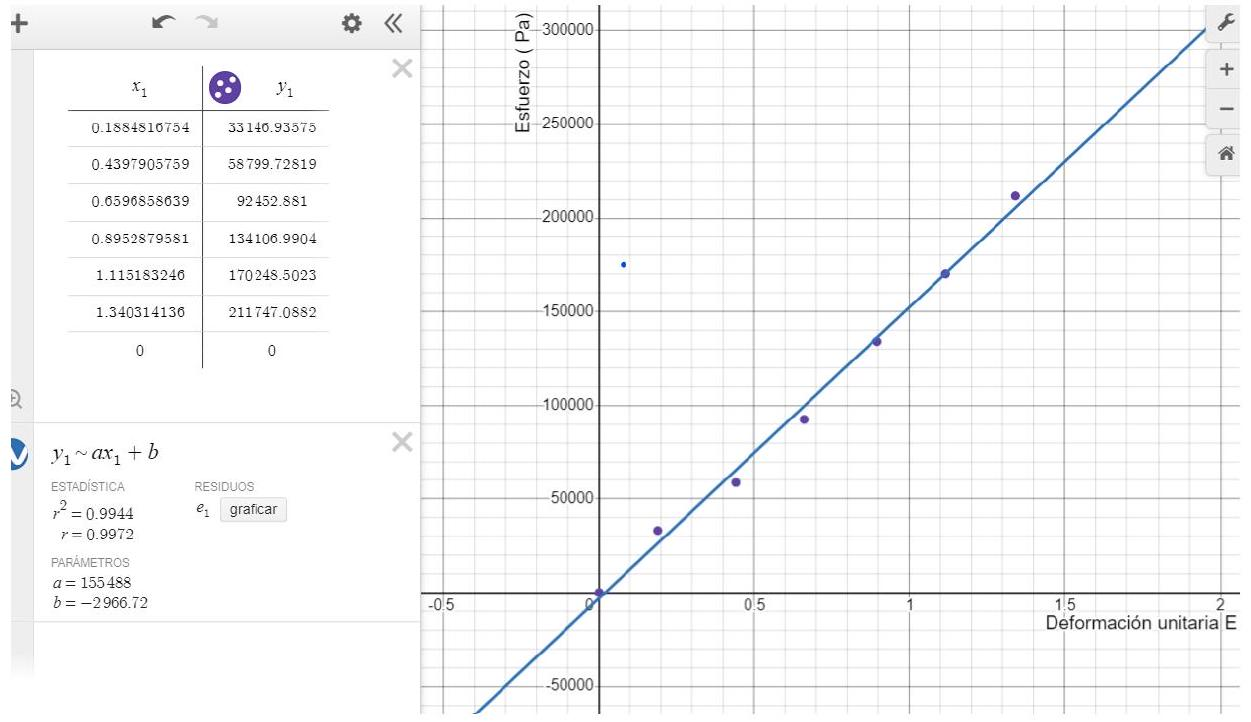
\includegraphics[max width=\textwidth, center]{2025_04_28_5f0b00b867417d4cd835g-4}
\end{itemize}

Figura 9: Gráfico $\sigma$ vs $\varepsilon$ para el resorte

De la gráfica presente en la figura 8 , tenemos:

\begin{itemize}
  \item Se observa una relación aproximada proporcional entre esfuerzo y deformación unitaria(al incluir al origen en la gráfica).
  \item De lo anterior, podemos asumir que la constante de proporcionalidad viene a ser el módulo de Young por tracción del material del resorte.
  \item Según la gráfica, el valor del módulo de Young por tracción es $Y=155488 \mathrm{~Pa}$.
\end{itemize}

Para la gráfica $\sigma$ vs $\varepsilon$ en el caso de la liga, tenemos la siguiente tabla:

\begin{center}
\begin{tabular}{|l|l|l|l|l|l|}
\hline
$\mathrm{N}^{\circ}$ & Peso(N) & $\mathrm{S}\left(10^{-6} m^{2}\right)$ & $\Delta \mathrm{L}\left(10^{-3} \mathrm{~m}\right)$ & $\sigma(\mathrm{Pa})$ & $\varepsilon$ \\
\hline
1 & 4.915 & 80.300 & 22 & 61205.604 & 0.074 \\
\hline
2 & 7.413 & 78.771 & 38 & 94113.293 & 0.128 \\
\hline
3 & 9.855 & 77.868 & 50 & 126561.951 & 0.169 \\
\hline
4 & 12.354 & 74.464 & 80 & 165902.087 & 0.270 \\
\hline
5 & 14.770 & 73.660 & 102 & 200516.104 & 0.345 \\
\hline
6 & 17.269 & 70.862 & 130 & 243691.196 & 0.439 \\
\hline
\end{tabular}
\end{center}

Cuadro 5: Valores procesados de la tabla de carga para la liga

Las incertidumbres $\Delta a$ y $\Delta D$ tienen el mismo valor de $\Delta p$ debido a que se obtuvo de mediciones con el vernier, mientras que a $\Delta(\Delta L)$ le corresponde $\Delta \ell$.

\begin{center}
\begin{tabular}{|l|l|l|l|l|l|}
\hline
$\mathrm{N}^{\circ}$ & Peso(N) & $\mathrm{S}\left(10^{-6} m^{2}\right)$ & $\Delta \mathrm{L}\left(10^{-3} \mathrm{~m}\right)$ & $\sigma(\mathrm{Pa})$ & $\varepsilon$ \\
\hline
5 & 14.770 & 72.577 & 122 & 203507.6774 & 0.412 \\
\hline
4 & 12.354 & 74.880 & 95 & 164980.409 & 0.321 \\
\hline
3 & 9.855 & 77.804 & 66 & 126666.058 & 0.223 \\
\hline
2 & 7.413 & 78.899 & 47 & 93960.611 & 0.159 \\
\hline
1 & 4.915 & 81.324 & 36 & 60434.927 & 0.122 \\
\hline
\end{tabular}
\end{center}

Cuadro 6: Valores procesados de la tabla de descarga para la liga


*Falta insertar grafica*

Figura 10: Gráfica $\sigma$ vs $\varepsilon$

De las dos tablas y el gráfico anteriores, se rescata lo siguiente:

\begin{itemize}
  \item Los esfuerzos y deformaciones unitarias por tracción son diferentes respecto a carga y descarga debido al comportamiento elástico de la liga(demora en reponerse).
  \item No hay módulo elástico ni en carga ni en descarga debido a la relación no lineal entre esfuerzo y deformación unitaria por tracción.
\end{itemize}
